% Original book p67; original base PDF p71; input PDF p92; p067_s08 三、2（第3图）
% Role: question; original field: diagrams[0].tikz
% Compile with XeLaTeX from this figures/ directory.
\documentclass[12pt,tikz,border=5pt]{standalone}
\usepackage{fontspec}
\setmainfont[Path=../fonts/]{DroidSansFallback.ttf}
\setsansfont[Path=../fonts/]{DroidSansFallback.ttf}
\usepackage{amsmath,amssymb}
\usepackage{tikz}
\usetikzlibrary{calc,angles,quotes,arrows.meta,decorations.pathreplacing,decorations.pathmorphing,decorations.markings,patterns,positioning,fit,backgrounds,matrix,intersections,shapes.geometric}
\begin{document}
\color{black}
\tikzset{every picture/.append style={color=black}}
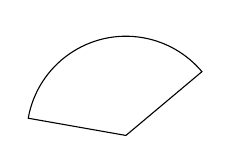
\begin{tikzpicture}[scale=.9]\draw(0,0)--(170:1.4)arc(170:40:1.4)--cycle;\end{tikzpicture}

\end{document}
